\documentclass[tikz,border=11pt]{standalone}
\usetikzlibrary{arrows.meta, positioning, calc, math, trees}

\begin{document}

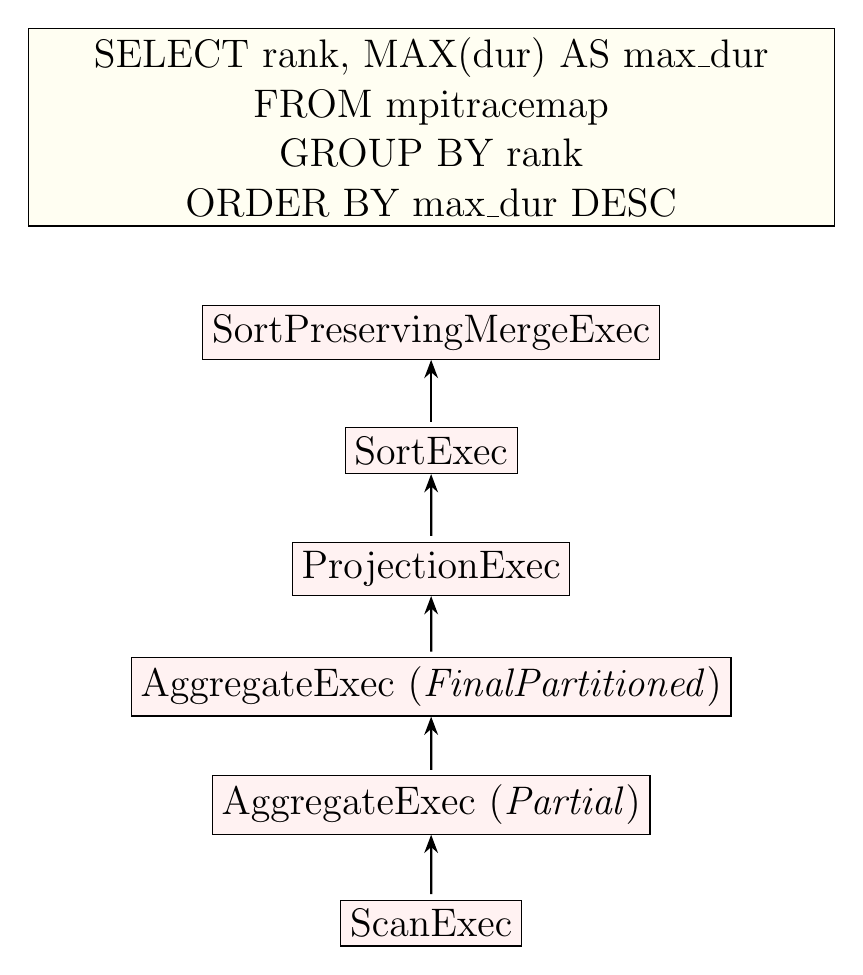
\begin{tikzpicture}[
		every node/.style={font=\Large, rectangle, thin, fill=red!5, draw=black},
    edge from parent/.style={draw, thick, {Stealth-}, shorten >=2pt}
	]
  \node (root) {SortPreservingMergeExec}
	child {
			node {SortExec}
			child {
					node {ProjectionExec}
					child {
							node {AggregateExec (\emph{FinalPartitioned})}
							child {
									node {AggregateExec (\emph{Partial})}
									child {node {ScanExec}}
								}
						}
				}
		};

  % \node [above=of root-0] {acbd};
  % \draw[->] (root) -- (-1, -1);
  \node [
    above=1cm of root,
    text width=10cm,
    align=center,
    fill=yellow!5
    ] {
      SELECT rank, MAX(dur) AS max\_dur \\
      FROM mpitracemap \\
      GROUP BY rank \\
      ORDER BY max\_dur DESC \\
    };
\end{tikzpicture}


\end{document}
